\chapter{多分类学习的可学习性}
\label{chap:multiclass-learnability}

上一章的二分类学习基本定理表明，对二分类假设空间，VC维有限、一致收敛、可实现PAC可学习和不可知PAC可学习四者相互等价。于是只要判断VC维是否有限，就同时知道风险能否被统一估计准确、学习能否成功。本章考察标签多于两类时，这一结论是否仍然成立。

二分类与多分类的差别在于，假设在一个输入上改变预测时可以改成什么。二分类假设只能从一个标签改为另一个；多分类假设可以改为其余任何一个标签。标签集合扩大后，有限输入上可能出现更多种预测组合，但实际能实现多少种仍取决于假设空间，不能只由标签数判断。因此，VC维所依赖的“两个标签的全部组合”需要换一种计数方式；上一章由同一个维度同时刻画一致收敛和可学习性的结论，也需要重新检验。

检验的结果取决于标签是否有限。标签有限时，预测计数可以推广到多类，二分类中的等价关系原样保留。标签无限时，计数失效，而且“能否把所有假设的风险同时估计准确”与“是否存在成功的学习算法”会分成两个不同的问题，需要两个不同的维度分别回答；后一个问题的答案还要求允许学习算法输出$\mathcal H$以外的分类器，也就是第~\ref{sec:learning-problem}节所说的非恰当学习。统计上能学习之后，仍要像上一章一样追问：训练和预测能否由总会停机的程序完成。

本章的设定只把第~\ref{sec:learning-problem}节中的二元标签换成有限或无限的标签集$Y$，其余保持不变：每条观测由输入和标签组成，样本独立同分布，采用零一损失，学习成功的标准仍是上一章的可实现PAC和不可知PAC。

\section{从二分类到多分类}
\label{sec:multiclass-setting}

把邮件标签扩展为正常、广告、诈骗三类。输入$x$仍是邮件特征，假设$h(x)$给出一个类别，只要与真实类别$y$不同就计一次错误。形式上，以$X$和$Y$为输入空间和标签空间，非空的$\mathcal H\subseteq Y^X$为假设空间，对联合分布$\mathcal P$和独立同分布样本$S=((x_i,y_i))_{i=1}^n$，定义~\ref{def:general-population-risk}与定义~\ref{def:general-empirical-risk}在零一损失下写成
\begin{equation}
 R_{\mathcal P}(h)=\mathbb P_{(x,y)\sim\mathcal P}\{h(x)\neq y\},\qquad
 \hat R_S(h)=\frac1n\sum_{i=1}^n\mathbb I\{h(x_i)\neq y_i\}.
 \label{eq:multiclass-risk}
\end{equation}
全章固定这一计分方式：预测正确计0，预测错误计1，错成哪一类都一样。可实现PAC要求在存在零风险假设时输出风险小的分类器，不可知PAC要求输出的风险接近$\mathcal H$中的最低风险，两者的量词次序与第~\ref{sec:pac-learning}节相同。统计定理仍需满足第~\ref{sec:learning-problem}节的可测性与可分性条件。

处理多分类的一个直接思路，是把它化归为上一章已经解决的二分类。标签有限时，可以先把每个类别编码成若干二进制位，例如对三类取
\[
 \text{正常}\longleftrightarrow(0,1),\qquad
 \text{广告}\longleftrightarrow(1,0),\qquad
 \text{诈骗}\longleftrightarrow(1,1).
\]
于是，每条带标签的邮件给出两个二分类任务的标签；例如一封广告邮件在第一位上的标签为1，在第二位上的标签为0。在同一批邮件上分别训练两个二分类器$b_1$和$b_2$，对新邮件先得到$(b_1(x),b_2(x))$，再按编码表解码成类别；不对应任何类别的编码$(0,0)$事先约定解码为“正常”。由于不同类别的编码互不相同，两位都预测正确时就能恢复正确类别，多分类问题由此转化为两个二分类问题。

一般地，当$2\leq K=|Y|<\infty$时，用$L=\lceil\log_2K\rceil$位给各类别分配互不相同的编码$c:Y\to\{0,1\}^L$，以$c_j(y)$记第$j$位。第$j$个二分类任务所用的假设空间，应由原假设空间在第$j$位上的投影得到，即把每个$h$的输出编码后只看第$j$位：
\[
 \mathcal B_j=\{x\mapsto c_j(h(x)):h\in\mathcal H\},\qquad 1\leq j\leq L.
\]
我们称$\mathcal B_j$为第$j$位的位空间。每一位的标签是二元的，但位空间本身仍可能很复杂；二分类的分布无关PAC要求VC维有限，编码本身并不能保证位空间满足这一条件。（若$K=1$，只有一个标签，常量预测就是零风险规则，无须拆分。）

先看可实现情形。若$h^\star\in\mathcal H$的风险为零，则$c_j\circ h^\star$属于第$j$个位空间，并且几乎处处预测出正确的位标签$c_j(y)$，所以每个位任务也都是可实现的。若每个位空间$\mathcal B_j$都PAC可学习，记学到的二分类器$b_j$在第$j$位上的错误率为
\[
 e_j=\mathbb P_{(x,y)\sim\mathcal P}\{b_j(x)\neq c_j(y)\}.
\]
以$\tilde h$记由各位预测解码得到的分类器。各位都预测正确时，类别一定正确；所以类别出错时，至少有一位出错，类别风险不超过各位错误率之和：
\[
 R_{\mathcal P}(\tilde h)\leq\sum_{j=1}^L e_j.
\]
这个不等式本身就是一次并集界：“类别出错”包含在“某一位出错”的并集中。于是，只要把每一位的风险目标定为$\varepsilon/L$、失败概率定为$\delta/L$，就有$\sum_je_j\leq\varepsilon$；而某一位学习失败的概率至多为$L\cdot\delta/L=\delta$，这是对失败事件的第二次并集界。合起来，以至少$1-\delta$的概率，类别风险至多为$\varepsilon$。以$m_{\mathcal B_j}(\varepsilon,\delta)$记位空间$\mathcal B_j$的可实现PAC样本量。各位可以共用同一份样本，也不要求它们的错误相互独立，只需样本量同时满足各位的要求：
\[
 n\geq\max_{1\leq j\leq L}
 m_{\mathcal B_j}(\varepsilon/L,\delta/L).
\]
解码得到的分类器不一定属于原假设空间$\mathcal H$，所以这是一种非恰当学习。

在不可知情形下，逐位学习不一定得到原任务的最优分类器。沿用上面的三类编码，设所有邮件的输入都相同，正常、广告、诈骗出现的概率分别为0.40、0.35、0.25，假设空间只含三个常量假设。第一位为1的概率是$0.35+0.25=0.60$，第二位为1的概率是$0.40+0.25=0.65$，所以每一位单独取最优都应预测1，解码后得到“诈骗”，类别风险为0.75；而直接预测“正常”的风险只有0.60。即使所有概率都已知，逐位取最优也选错了类别。原因在于两个目标不同：逐位学习分别降低每一位的错误率，多类零一损失只看整个类别是否正确。把正常邮件判为广告时，编码$(0,1)$变为$(1,0)$，两位都错，逐位错误计2次，类别错误只计1次；两种计数方式下的最优预测因而可能不同。

由此可见，编码只提供了一种构造学习算法的办法：要得到学习保证，还需控制各位空间的复杂度并合并各位的风险，而且这一保证只在可实现情形下成立。标签无限时，固定位数的编码无法区分无限多个类别，这种归约根本无法使用。因此需要换一条路：直接分析原假设空间在有限输入上能给出怎样的预测组合。

为此首先要确定多分类中“打散”的含义。二分类中，输入集被打散是指假设空间在这些输入上实现了全部$2^m$种预测。一种直接的推广是要求在$m$个输入上实现全部$|Y|^m$种预测，但这个要求过严。设三类邮件问题中的假设空间只会输出“正常”和“广告”，从不输出“诈骗”，并且把这两个标签看作0和1后，它是一个VC维无穷的二分类空间。由上一章的基本定理，这个空间不是PAC可学习的，那里的下界构造只用到两个标签，可以原样搬过来。可是它在任何一个输入上都实现不了“诈骗”，按全部$|Y|^m$种预测的要求，连单个输入都打散不了，复杂度会被记为0。

问题出在要求每个输入用遍所有标签。困难其实只需要每个输入上有两个可选答案，并且这些选择可以在各输入之间自由组合。因此更合适的做法是先为每个输入指定两个不同的标签，再问假设空间能否在每个输入上独立地取这两个标签中的任意一个。能做到这一点的最大输入数，称为\term{Natarajan维}（Natarajan dimension）。在上面的例子中，给每个输入都指定$\{\text{正常},\text{广告}\}$，Natarajan维就等于那个二分类空间的VC维。

\section{有限标签空间及Natarajan维的边界}
\label{sec:multiclass-dimensions}

本节限定标签有限，$2\leq K=|Y|<\infty$。分析路线与上一章平行：先用Natarajan维限制假设空间在有限输入上的预测个数，再沿用上一章的对称化论证得到一致收敛，最后由ERM的风险比较得到可学习性。

\subsection{Natarajan维}

第~\ref{def:natarajan-dimension}定义与式~\eqref{eq:natarajan-shattering}已规定组合量词；本节说明它怎样进入有限标签的风险估计。

具体地，对互异输入$x_1,\ldots,x_m$，Natarajan打散先为每个$x_i$指定两个不同的标签$a_i\neq b_i$，再要求对每个选择向量$s\in\{0,1\}^m$，都有某个假设在$s_i=0$的输入上预测$a_i$、在$s_i=1$的输入上预测$b_i$。不同输入可以指定不同的标签对，但标签对一经指定，就不能随要实现的组合改变（组合定义见第~\ref{sec:comb-fixed-label-pairs}节）。本章以$d_N(\mathcal H)$记能被Natarajan打散的有限输入集大小的上确界。

例如在两封邮件$x_1,x_2$上，给$x_1$指定$\{\text{正常},\text{广告}\}$，给$x_2$指定$\{\text{广告},\text{诈骗}\}$。要打散$\{x_1,x_2\}$，假设空间必须同时含有在这两处分别预测（正常，广告）、（正常，诈骗）、（广告，广告）、（广告，诈骗）的假设；至于它们在其他输入上预测什么，以及是否还会在$x_1,x_2$上预测别的标签，都不影响判断。
% 旧公式位置保留为导航锚点，不再重复通用定义式。
\phantomsection\label{eq:learning-natarajan-shattering}

这个定义本身并不要求标签有限。在二分类中，每个输入上只能指定$\{0,1\}$这一对标签，所以Natarajan打散就是打散，Natarajan维等于VC维。Natarajan维为0，说明每个输入上的预测都唯一；若能被打散的输入集没有有限上界，维度为无穷。下面用这个维度控制预测个数。

\subsection{有限标签的一致收敛}

与上一章一样，固定输入后，把在这些输入上预测相同的假设视为同一种。令
\[
 V(x_1,\ldots,x_m)
 =\{(h(x_1),\ldots,h(x_m)):h\in\mathcal H\}.
\]
再对输入的选择取上确界，得到生长函数
\[
 \Pi_{\mathcal H}(m)=\sup_{(x_1,\ldots,x_m)\in X^m}|V(x_1,\ldots,x_m)|.
\]
这与第~\ref{sec:binary-growth-sauer}节二分类的计数相同，区别只在于每个坐标可以取$K$个标签。在二分类中，Sauer--Shelah引理用VC维限制预测个数；在有限标签的多分类中，Natarajan维起同样的作用。

% 保留旧位置锚点；这里直接使用组合计数结论。
\phantomsection\label{thm:learning-multiclass-growth-bound}
当$2\leq K=|Y|<\infty$且$d=d_N(\mathcal H)<\infty$时，记$q=K(K-1)/2$为不同的无序标签对的个数。对每个整数$m\geq0$，多类的计数界（Natarajan引理）给出
\[
 \Pi_{\mathcal H}(m)\leq G_{d,K}(m)
 :=\sum_{j=0}^{\min\{d,m\}}\binom mj q^j
\]
在学习问题中，$G_{d,K}(2n)$将控制原样本与副样本合在一起的$2n$个输入上不同损失模式的个数，从而进入对称化之后的失败概率。

二分类时$q=1$且$d_N=\operatorname{VC}(\mathcal H)$，求和式回到Sauer--Shelah引理中的$\sum_{j=0}^{\min\{d,m\}}\binom mj$。多类时多出的因子$q^j$计入了一个事实：在每个参与二元选择的坐标上，标签对可以是$q$种中的任意一种。

这个界的作用在于它随$m$的增长速度。全部可能的预测有$K^m$种，随$m$指数增长；而由$\binom mj\leq m^j$，当$m\geq1$时
\[
 G_{d,K}(m)\leq(d+1)q^dm^d,
\]
固定$d$和$K$后只按$m^d$的多项式增长。样本标签固定后，相同的预测向量给出相同的损失向量，所以这个计数也控制了经验风险分析中需要区分的情况数。上一章的证明正是靠“情况数只按多项式增长、而每种情况的偏差概率按指数衰减”取胜，这里可以沿用同一论证。

% 避免短定理在页末仅留下标题和半句条件。
\begingroup
\tcbset{lines before break=4}
\begin{theorem}[有限标签的一致收敛保证]
\label{thm:finite-label-uniform-convergence}
设$(X,\mathcal X)$为可测空间，离散标签空间$Y$满足
$2\leq|Y|=K<\infty$，$\mathcal H\subseteq Y^X$是由可测分类器组成的非空集合，
$d=d_N(\mathcal H)<\infty$，并令
\[
 G_{d,K}(m)=\sum_{j=0}^{\min\{d,m\}}\binom mj
 \left(\frac{K(K-1)}2\right)^j.
\]
假定零一损失类$\mathcal L_{\mathcal H}
=\{(x,y)\mapsto\mathbb I\{h(x)\neq y\}:h\in\mathcal H\}$中的每个函数均可测，
并存在可数子类$\mathcal L_0\subseteq\mathcal L_{\mathcal H}$，使每个
$f\in\mathcal L_{\mathcal H}$都是$\mathcal L_0$中某个函数序列的逐点极限。
设$\mathcal P$为$X\times Y$上的任意联合分布，$n\geq1$，
$S=((x_i,y_i))_{i=1}^n\sim\mathcal P^n$，并记
\[
 R_{\mathcal P}(h)=\mathbb P_{(x,y)\sim\mathcal P}\{h(x)\neq y\},\qquad
 \hat R_S(h)=\frac1n\sum_{i=1}^n\mathbb I\{h(x_i)\neq y_i\}.
\]
则对任意$\delta\in(0,1)$，以关于$S\sim\mathcal P^n$至少$1-\delta$的概率，
\begin{equation}
 \sup_{h\in\mathcal H}|R_{\mathcal P}(h)-\hat R_S(h)|
 \leq\sqrt{\frac8n\log\frac{4G_{d,K}(2n)}{\delta}}.
 \label{eq:finite-label-uniform-bound}
\end{equation}
\end{theorem}
\endgroup

\begin{proof}
证明沿用上一章的三步，只在计数一步换用$G_{d,K}$。取$\eta>0$且$n\eta^2\geq2$。

第一步是对称化。另取独立副样本$S'$，当$n\eta^2\geq2$时，“某个假设的总体风险与经验风险相差超过$\eta$”的概率，至多是“某个假设在$S$与$S'$上的经验风险相差超过$\eta/2$”的概率的两倍。这样，未知的总体风险就被换成了可以数的经验量。

第二步是计数。$S$与$S'$共有$2n$个输入，标签已经固定；在这些输入上预测相同的假设给出相同的损失向量，所以只需考虑至多$\Pi_{\mathcal H}(2n)\leq G_{d,K}(2n)$个损失向量。

第三步是随机交换与并集界。对固定的损失向量，逐对独立地以各一半的概率交换$(z_i,z_i')$，两份经验风险之差变成$\frac1n\sum_i\sigma_ic_i$，其中$\sigma_i$为随机符号，$c_i\in\{-1,0,1\}$。由Hoeffding不等式，它的绝对值超过$\eta/2$的概率至多$2e^{-n\eta^2/8}$。对至多$G_{d,K}(2n)$个损失向量求并集界，再乘上第一步的因子2，得到
\[
 \mathbb P\!\left\{\sup_h|R_{\mathcal P}(h)-\hat R_S(h)|>\eta\right\}
 \leq4G_{d,K}(2n)e^{-n\eta^2/8}.
\]
令右侧等于$\delta$，解出$\eta=\sqrt{(8/n)\log(4G_{d,K}(2n)/\delta)}$。此时$n\eta^2=8\log(4G_{d,K}(2n)/\delta)\geq8\log4>2$，第一步的条件自动满足。若这个$\eta$超过1，结论因零一风险之差不超过1而平凡成立。
\end{proof}

这里$\mathcal P$可以是任意联合分布，不要求各类别等概率出现。固定$d,K,\delta$，式~\eqref{eq:finite-label-uniform-bound}根号内的$\log G_{d,K}(2n)$只按$d\log n$增长，除以$n$后趋于零；这个上界又不含$\mathcal P$，因此得到分布无关的一致收敛。类别数的影响也可以读出来：当$1\leq d\leq2n$时，$G_{d,K}(2n)\leq q^d(2en/d)^d$，取对数得$d\log q+d\log(2en/d)$，而$\log q\leq2\log K$，所以类别数$K$只以$d\log K$的量级进入根号。

\subsection{有限标签的可学习性}

有了所有假设风险的同时估计，就可以像上一章一样分析ERM的输出：从输出和参照假设的总体风险换到经验风险，各产生一次偏差。反方向上，Natarajan打散可以用来构造使任何算法都失败的分布。两者合起来，得到有限标签下的双向刻画。

\begin{theorem}[有限标签的可学习性刻画]
\label{thm:finite-label-learnability}
设$(X,\mathcal X)$为可测空间，离散标签空间$Y$满足
$2\leq|Y|=K<\infty$，$\mathcal H\subseteq Y^X$是由可测分类器组成的非空集合，
并采用零一损失。假定损失类
$\mathcal L_{\mathcal H}
=\{(x,y)\mapsto\mathbb I\{h(x)\neq y\}:h\in\mathcal H\}$中的每个函数均可测，
且存在可数子类$\mathcal L_0\subseteq\mathcal L_{\mathcal H}$，使每个
$f\in\mathcal L_{\mathcal H}$都是$\mathcal L_0$中某个函数序列的逐点极限。
学习算法均为可测映射，训练样本均为$S\sim\mathcal P^n$，成功概率同时计入样本抽取
和算法的内部随机性。在这一分布无关设定中，以下命题等价：
\begin{enumerate}
 \item $d_N(\mathcal H)<\infty$；
 \item 零一损失满足分布无关的一致收敛；
 \item $\mathcal H$不可知PAC可学习；
 \item $\mathcal H$可实现PAC可学习。
\end{enumerate}

设$d=d_N(\mathcal H)<\infty$，并令
\[
 G_{d,K}(m)=\sum_{j=0}^{\min\{d,m\}}\binom mj
 \left(\frac{K(K-1)}2\right)^j.
\]
对任意$\varepsilon,\delta\in(0,1)$、任意$X\times Y$上的联合分布$\mathcal P$，
若$n\geq1$且
\[
 n\geq\frac{32}{\varepsilon^2}\log\frac{4G_{d,K}(2n)}{\delta},
\]
则任意以概率1输出
$A(S)\in\argmin_{h\in\mathcal H}\hat R_S(h)$的可测ERM，在
$S\sim\mathcal P^n$及其内部随机性的联合概率下，以至少$1-\delta$的概率满足
\[
 R_{\mathcal P}(A(S))\leq\inf_{h\in\mathcal H}R_{\mathcal P}(h)+\varepsilon.
\]
\end{theorem}

\begin{proof}
先证有限Natarajan维推出学习成功。题设的样本量条件正是使式~\eqref{eq:finite-label-uniform-bound}右端不超过$\varepsilon/2$的条件，所以以至少$1-\delta$的概率，所有假设的偏差同时不超过$\varepsilon/2$。在这个事件内，对任意参照假设$h$，依次用偏差界、ERM的最优性和偏差界：
\begin{align*}
 R_{\mathcal P}(A(S))&\leq\hat R_S(A(S))+\varepsilon/2\\
 &\leq\hat R_S(h)+\varepsilon/2\\
 &\leq R_{\mathcal P}(h)+\varepsilon.
\end{align*}
对参照取下确界得不可知PAC。可实现分布属于这一允许族，因此也得到可实现PAC。

再证反方向：若Natarajan维无穷，则可实现PAC也不成立。对任意样本量$n$，取被Natarajan打散的$2n$个输入及各自指定的标签对，令输入在这$2n$点上均匀分布，目标在每个点的标签对中独立地等概率选一个。由打散的定义，每个这样的目标都由某个假设实现，所以对应的分布是可实现的。$n$次抽样至多见到$n$个不同的点，至少一半的点未被见到；在未见点上，目标标签与样本独立且在两个标签间等概率，任何算法在那里预测正确的概率都至多$1/2$。因此，对随机目标取平均，任意算法的期望风险至少$\frac12\cdot\frac12=1/4$。

平均值至少$1/4$，说明至少有一个固定的目标使期望风险$\mathbb ER\geq1/4$。记$p=\mathbb P\{R>1/8\}$，由$R\leq1$得$\mathbb ER\leq\frac18(1-p)+p\leq\frac18+\frac78p$，于是$p\geq1/7$。取$\varepsilon=1/8$、$\delta=1/8$，任何样本量都达不到要求，这违反分布无关的可实现PAC。
\end{proof}

定理中的样本量条件两边都含$n$：左边按$n$线性增长，右边的$\log G_{d,K}(2n)$只按$d\log n$增长，所以足够大的$n$总能满足它，满足条件的最小$n$就是一个可用的样本量。这个样本量只是充分条件，并不声称达到两种PAC设定下的最优样本复杂度。

必要性的证明只用到每个输入上指定的两个标签，并没有用到标签总数有限，所以对任意标签空间$Y$，PAC可学习都要求Natarajan维有限。标签有限只在另一个方向，即预测计数中起作用。

\subsection{Natarajan维在无限标签空间下的局限}
\label{sec:multiclass-erm-limitations}

标签无限时，标签对的个数$q=\binom K2$不再有限，上面的计数界失效。不过，证明方法失效不等于结论不成立。要说明在无限标签下Natarajan维有限不足以保证可学习，必须实际构造一个Natarajan维有限、却不可学习的假设空间。

先看两个输入上的一个小例子。设限制在这两个输入上的假设类恰好给出以下六种预测：
\[
 (a,u),\ (b,u),\ (b,v),\ (c,v),\ (c,w),\ (a,w),
\]
其中$a,b,c$互不相同，$u,v,w$互不相同。这六个向量有一个共同特点：对每个向量和每个坐标，类中都有另一个向量只在该坐标上与它不同，我们称后者为前者在该坐标上的邻居。例如，$(a,u)$在第一坐标上的邻居是$(b,u)$，在第二坐标上的邻居是$(a,w)$。这意味着，即使知道其中一个坐标的标签，另一个坐标仍有两个可能的标签：已知第二坐标为$u$时，第一坐标可以是$a$或$b$。

另一方面，这个类的Natarajan维只有1。要打散两个坐标，需要在第一坐标选两个标签、在第二坐标选两个标签，使四种组合都出现；也就是说，第一坐标的两个标签各自都要能与同样两个第二坐标标签搭配。但在这个类中，$a$只与$u,w$搭配，$b$只与$u,v$搭配，$c$只与$v,w$搭配，任意两个第一坐标标签只有一个共同的搭配对象，凑不出四种组合。可见，Natarajan维小并不排除每个坐标上都存在不确定性。这个有限类本身是可学习的；要构造不可学习的反例，还需要在任意多个坐标上具有同样结构的例子。

图~\ref{fig:learning-theory-ds-neighbors}把六个向量之间的邻居关系画成一个环。每个顶点连着一条只改变第一坐标的边和一条只改变第二坐标的边，所以两个坐标上的不确定性同时存在；而这种邻居关系并不要求某两对标签的四种组合全部出现。

\begin{figure}[htbp]
  \centering
  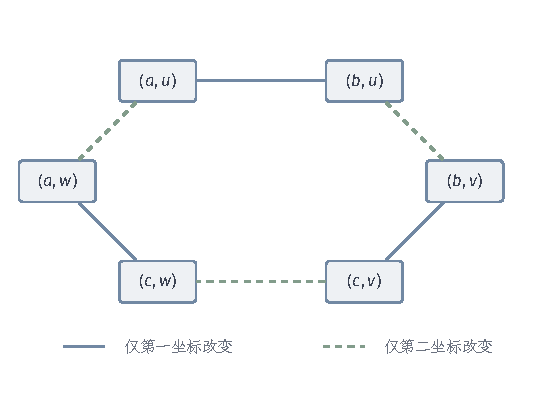
\includegraphics[width=93.405mm]{figures/06-foundations/02-learning-theory/tikz/learning-theory-ds-neighbors/figure.pdf}
  \caption{六种预测的坐标邻接环。顶点为上文的六个向量，蓝色实线仅改变第一坐标，绿色虚线仅改变第二坐标；边没有方向。每个顶点在两个坐标上分别有邻居，却不存在固定两对标签的完整四种组合。因而这个两输入函数类的Natarajan维为1，后文分析的DS维为2；它仍是可学习的有限类，不能单独证明不可学习性。}
  \label{fig:learning-theory-ds-neighbors}
\end{figure}

要由这种不确定性得到不可学习性，需要对任意多个坐标都有同类构造。下面的引理给出这样的构造；其中把$V_m$中的向量看作坐标集$\{1,\ldots,m\}$上的函数，这样才能谈论它的Natarajan维。

\begin{lemma}[低Natarajan维的局部邻接构造]
\label{lem:low-natarajan-pseudocubes}
对每个整数$m\geq1$，把$Y_m^m$中的向量视为定义在坐标集
$\{1,\ldots,m\}$上的分类函数。存在非空有限标签集$Y_m$及有限非空函数集合
$V_m\subseteq Y_m^{\{1,\ldots,m\}}$，使
\begin{enumerate}
 \item $d_N(V_m)=1$；
 \item 对任意$v\in V_m$和$i\in\{1,\ldots,m\}$，存在$u\in V_m$满足
 \[
 u_i\neq v_i,\qquad u_j=v_j\quad(j\neq i).
 \]
\end{enumerate}
\end{lemma}

这个引理由Brukhim等人的组合拓扑构造给出\scite{brukhim2022multiclass}，本章不展开证明。它同时具有两条性质：一方面，在指定的标签对之间无法自由选择（Natarajan维为1）；另一方面，每个向量在每个坐标上都有邻居。下面把各个$m$对应的构造拼成同一个假设空间，证明它不可学习。

\begin{theorem}[无限标签下有限Natarajan维并不充分]
\label{thm:natarajan-infinite-counterexample}
在输入与标签均取离散$\sigma$代数、训练样本独立同分布并采用零一损失的设定中，
存在可数预测输入空间$X$、可数标签空间$Y$和非空假设空间
$\mathcal H\subseteq Y^X$，使$d_N(\mathcal H)=1$，但不存在对所有
$\mathcal H$可实现联合分布都具有分布无关可实现PAC保证的可测学习算法。
\end{theorem}

\begin{proof}
对各$m$取引理~\ref{lem:low-natarajan-pseudocubes}中的$V_m$，把输入组成互不相交的块$C_m=\{(m,1),\ldots,(m,m)\}$，令$X=\bigcup_{m\geq1}C_m$。局部标签加块编号写为$(m,y)$，因此$(2,a)$与$(3,a)$是不同类别。另设普通标签$\star$表示不在所选块，它不同于全部$(m,y)$，并非未知、缺失或任意值。标签总空间为
\[
 Y=\{\star\}\cup\bigcup_{m\geq1}(\{m\}\times Y_m).
\]
每个$v\in V_m$扩展为整个预测输入空间上的假设
\[
 h_{m,v}(r,i)=
 \begin{cases}
 (m,v_i),&r=m,\\
 \star,&r\neq m.
 \end{cases}
\]
例如$h_{2,v}$只在$C_2$使用局部答案，其他块均答$\star$。以全部$h_{m,v}$组成$\mathcal H$，各维困难块便属于同一个固定空间。

先算Natarajan维。设两点被Natarajan打散。每个点的标签对由两个不同标签组成，所以至少含一个非$\star$标签。若两点在不同块，要让两点同时取各自的非$\star$标签，就需要一个假设在两个块上都输出非$\star$标签，而每个$h_{m,v}$只在自己的块上这样做，矛盾。若两点在同一块$C_m$，且某点的标签对含$\star$，考虑该点取$\star$、另一点取其非$\star$标签的组合：在该点输出$\star$的假设来自其他块，在整个$C_m$上都输出$\star$，实现不了这个组合；若两个标签对都不含$\star$，则需要$V_m$在两个坐标上被Natarajan打散，与$d_N(V_m)=1$矛盾。单点可以被打散：同一点上可取局部标签或$\star$。所以$d_N(\mathcal H)=1$。

下面说明$\mathcal H$不可学习。对给定的$n$取$m=2n$，令输入在$C_m$上均匀分布，目标从有限集$V_m$中均匀抽取，标签由$h_{m,v}$给出，因此分布可实现。考虑一个未被抽到的坐标$i$。学习器在该坐标上的预测只依赖抽到的位置、这些位置上的标签和内部随机性；即使再把$i$以外全部坐标的真实标签告诉它，坐标$i$上的标签仍不确定。原因是，与其余坐标的标签都吻合的向量，两两在坐标$i$上取不同的标签，否则它们就是同一个向量；邻居条件保证这样的向量至少有两个；目标在$V_m$上均匀，条件在这些向量上仍然均匀。所以坐标$i$上的标签在至少两个不同值上等概率分布，学习器在那里的错误概率至少为$1/2$。

$n$次抽样至少遗漏$2n$个点中的一半，所以对目标、样本和算法的内部随机性取平均后，风险至少为$1/4$。接下来的论证与定理~\ref{thm:finite-label-learnability}的必要性部分相同：必有某个固定目标$v$的期望风险至少$1/4$，从而风险超过$1/8$的概率至少为$1/7$。每个样本量都存在这样的可实现分布，所以不存在统一的PAC样本量。
\end{proof}

这个例子说明，困难并不来自标签无限本身，而是Natarajan维有限不足以排除所有导致学习失败的结构。下一节把“同时估计准确所有假设的风险”与“存在成功的学习算法”分开，分别寻找刻画它们的维度。

\section{图维、DS维与一般标签空间}
\label{sec:general-multiclass-dimensions}
\label{sec:multiclass-sample-complexity}
在有限标签下，Natarajan维通过预测计数同时保证一致收敛和可学习性。去掉标签有限的条件后，第~\ref{sec:multiclass-erm-limitations}节给出了Natarajan维有限却不可学习的例子，这一联系不复存在。因此需要分别回答两个问题：同一份样本能否把所有假设的风险同时估计准确？是否存在某个算法能输出低风险的分类器？前者是对整个假设空间的要求，后者只涉及学习算法的输出。

对第一个问题，零一风险只关心预测是否等于真实标签，所以可以把每个假设换成取值0或1的损失函数，再对损失函数类使用上一章的VC维理论。对第二个问题，学习算法可以利用标签携带的更多信息，不必把所有风险都估计准确；需要刻画的是学习算法无法消除的不确定性，前面六种预测的例子已经给出了它的形状。

\subsection{一致收敛}

零一损失把所有错误一律计为1，风险只取决于预测是否等于真实标签。因此，要刻画的是一种二元能力：先为每个输入指定一个参考标签$f(x)$，再问假设空间能否任意指定在哪些输入上预测等于参考标签。\term{图打散}（graph shattering）要求：对这组输入的每个子集，都有某个假设恰好在这个子集的输入上预测为参考标签，在其余输入上预测为其他标签；预测不等于参考标签时具体取哪个标签，可以随子集不同而不同。名称中的“图”指函数的图像，即由输入与参考标签组成的点对集合，与由节点和边构成的图无关。写成条件，就是存在$f:C\to Y$，使对每个$B\subseteq C$都有$h\in\mathcal H$满足：$x\in B$时$h(x)=f(x)$，$x\in C\setminus B$时$h(x)\neq f(x)$。

例如对两封邮件取参考标签$f(x_1)=\text{正常}$、$f(x_2)=\text{广告}$。要图打散$\{x_1,x_2\}$，需要四个假设分别做到：两封都判对参考标签；只有$x_1$判为“正常”；只有$x_2$判为“广告”；两封都不等于参考标签。后三种情形中“不等于”可以取任何其他类别，例如第四种可以是（广告，诈骗），也可以是（诈骗，正常）。

能被图打散的有限输入集大小的上确界称为\term{图维}（graph dimension），记为$d_G(\mathcal H)$。它衡量的是假设空间能多自由地决定“在哪些输入上与参考标签一致”。比较两种打散：图打散只指定参考标签，不等于参考标签时取什么标签不受限制；Natarajan打散还指定了每个输入上的另一个标签，要求更严。所以能被Natarajan打散的输入集一定能被图打散，反之不然，即$d_N\leq d_G$。下面利用“等于或不等于参考标签”的二元模式，把图维转化为零一损失类的VC维。

为此把每个假设换成它的零一损失函数，组成$\mathcal L_{\mathcal H}=\{(x,y)\mapsto\mathbb I\{h(x)\neq y\}:h\in\mathcal H\}$。这些函数以输入和标签组成的点对为自变量，取值0或1，因而可以对它们谈论VC维。

\begin{theorem}[图维与一致收敛]
\label{thm:graph-uniform-convergence}
设$(X,\mathcal X)$为可测空间，$Y$为取离散$\sigma$代数的非空标签空间，
$\mathcal H\subseteq Y^X$是由可测分类器组成的非空集合，并令
\[
 \mathcal L_{\mathcal H}
 =\{(x,y)\mapsto\mathbb I\{h(x)\neq y\}:h\in\mathcal H\}.
\]
则$\operatorname{VC}(\mathcal L_{\mathcal H})=d_G(\mathcal H)$。
进一步假定$\mathcal L_{\mathcal H}$中的函数均可测，且存在可数子类
$\mathcal L_0\subseteq\mathcal L_{\mathcal H}$，使每个损失函数都是
$\mathcal L_0$中某个函数序列的逐点极限。此时$d_G(\mathcal H)<\infty$当且仅当：
对任意$\eta,\delta\in(0,1)$，存在不依赖联合分布$\mathcal P$的样本量
$m(\eta,\delta)$，使任意$n\geq m(\eta,\delta)$及
$S=((x_i,y_i))_{i=1}^n\sim\mathcal P^n$均满足
\[
 \mathbb P_{S\sim\mathcal P^n}\left\{
 \sup_{h\in\mathcal H}|R_{\mathcal P}(h)-\hat R_S(h)|\leq\eta
 \right\}\geq1-\delta,
\]
其中$R_{\mathcal P}$与$\hat R_S$均为零一损失风险。
\end{theorem}

\begin{proof}
关键在于：在点$(x,f(x))$上，损失$\mathbb I\{h(x)\neq f(x)\}$为0恰好表示$h$与参考标签一致。若以$f$图打散$C$，则对点集$\{(x,f(x)):x\in C\}$的每种0/1损失模式，取“损失为0的输入”作为$B$，图打散提供的假设就实现了这一模式，故$\operatorname{VC}(\mathcal L_{\mathcal H})\geq d_G(\mathcal H)$。

反过来，设损失类打散了点集$\{(x_i,y_i)\}$。其中不能有同一个$x$配两个不同的$y$：两处损失同时为0要求$h(x)$同时等于两个不同标签。所以这些输入互异，可以令$f(x_i)=y_i$，损失模式的0/1正好对应与参考标签一致/不一致，于是这些输入被图打散，$d_G(\mathcal H)\geq\operatorname{VC}(\mathcal L_{\mathcal H})$。两维相等后，上一章关于二值函数类的“VC维有限当且仅当一致收敛”即给出所述等价。
\end{proof}

于是，图维判定了整个假设空间的风险能否被同时估计准确。与上一章一样，“所有风险同时估计准确”的事件也覆盖ERM选出的输出，因此可以从“经验风险最小”推出“总体风险接近$\mathcal H$中的最低水平”。下面写出这一推论。

\begin{theorem}[一致收敛推出可学习性]
\label{thm:multiclass-uniform-pac}
设$(X,\mathcal X)$为可测空间，$Y$为离散标签空间，
$\mathcal H\subseteq Y^X$是由可测分类器组成的非空集合。采用零一损失，记
\[
 R_{\mathcal P}(h)=\mathbb P_{(x,y)\sim\mathcal P}\{h(x)\neq y\},\qquad
 \hat R_S(h)=\frac1n\sum_{i=1}^n\mathbb I\{h(x_i)\neq y_i\}.
\]
假定损失类中的函数均可测，并存在可数损失子类，使每个损失函数都是该子类中某个
函数序列的逐点极限；$\mathcal H$满足分布无关的一致收敛。对任意
$\varepsilon,\delta\in(0,1)$，若$n\geq1$足以使任意$X\times Y$上的联合分布
$\mathcal P$及样本$S\sim\mathcal P^n$满足
\[
 \mathbb P\!\left\{
 \sup_{h\in\mathcal H}|\hat R_S(h)-R_{\mathcal P}(h)|\leq\varepsilon/2
 \right\}\geq1-\delta,
\]
则任意以概率1输出
$A(S)\in\argmin_{h\in\mathcal H}\hat R_S(h)$的可测ERM学习算法$A$，均以至少
$1-\delta$的概率满足
\[
 R_{\mathcal P}(A(S))\leq\inf_{h\in\mathcal H}R_{\mathcal P}(h)+\varepsilon.
\]
概率同时来自$S\sim\mathcal P^n$和$A$的内部随机性。
因此，$\mathcal H$不可知PAC可学习，也可实现PAC可学习。
\end{theorem}

\begin{proof}
将每个$h$换成二值损失函数，经验最优比较保持不变。第~\ref{chap:binary-learnability}章的两次$\varepsilon/2$偏差分别用于输出和任意参照，得到总体超额至多$\varepsilon$；再对参照取下确界即为不可知PAC。可实现来源使该下确界为0，因而也满足可实现保证。
\end{proof}

所以，图维有限经由一致收敛和ERM推出可学习。但在无限标签下，图维有限并不是可学习的必要条件。

原因在于，一致收敛要求整个假设空间的风险都能被估计准确，而学习算法可能只需辨认出正确的目标。下面构造一个例子，其中标签本身就透露了目标是哪个假设：整个假设空间不满足一致收敛，却存在成功的学习算法。

取$X=\mathbb N$，把每个有限的自然数子集当作一个类别，再加一个与它们都不同的特殊标签$\star$，表示“输入不在目标集合中”。对每个有限集$A$定义
\begin{equation}
 h_A(x)=\begin{cases}A,&x\in A,\\\star,&x\notin A,\end{cases}
 \qquad\mathcal H_C=\{h_A:A\subset\mathbb N\text{有限}\}.
 \label{eq:cantor-class}
\end{equation}
在这个假设空间中，一个非$\star$的标签（例如$\{2,5\}$）直接写出了目标集合的全部成员。所以在可实现分布下，只要样本中出现一条非$\star$标签的观测，就能完全确定目标；若样本中的标签全是$\star$，就输出$h_{\varnothing}$。这里的标签是为说明问题而特意构造的，它携带了整条判定规则，与通常意义上表示语义类别的标签不同。

\begin{theorem}[可学习性不推出一致收敛]
\label{thm:multiclass-erm-separation}
令$X=\mathbb N$，标签空间$Y$由特殊标签$\star$与$\mathbb N$的所有有限子集组成，
二者均取离散$\sigma$代数。对每个有限$A\subseteq\mathbb N$定义
\[
 h_A(x)=\begin{cases}A,&x\in A,\\\star,&x\notin A,\end{cases}
 \qquad
 \mathcal H_C=\{h_A:A\subseteq\mathbb N\text{有限}\}.
\]
采用独立同分布抽样与零一损失。学习算法在样本出现非$\star$标签时，按样本顺序取第一个这样的标签$A$并输出$h_A$，
在所有标签均为$\star$时输出$h_{\varnothing}$；该算法使$\mathcal H_C$可实现PAC可学习。
另一方面，对大小为$n$且标签全为$\star$的样本，令
$A_S=\{1,\ldots,2n\}\setminus\{x_1,\ldots,x_n\}$并输出$h_{A_S}$；对其他样本，
在$h_{\varnothing}$及样本中出现的有限集合标签对应的假设之间，按预先固定的顺序选择
零一经验风险最小者。这个规则是确定性恰当ERM，却没有分布无关PAC保证。
此外，$\mathcal H_C$满足$d_N(\mathcal H_C)=1$及$d_G(\mathcal H_C)=\infty$，
因而不满足零一损失的一致收敛。
\end{theorem}

\begin{proof}
先证第一个算法成功。设目标为$h_A$，以$p=\mathcal P_X(A)$记输入落在$A$中的概率。样本中只要有一个输入落在$A$里，它的标签就是$A$本身，算法恢复出目标，风险为0；否则算法输出$h_{\varnothing}$，它恰好在$A$上出错，风险为$p$。所以风险超过$\varepsilon$只可能发生在$p>\varepsilon$且$n$个输入都没落在$A$中时，其概率为$(1-p)^n\leq(1-\varepsilon)^n\leq e^{-n\varepsilon}$。令它不超过$\delta$，样本量$n\geq\log(1/\delta)/\varepsilon$就够了，与分布无关。

再算两个维度。任意有限输入集$C$都能以全$\star$为参考标签被图打散：要恰在$B\subseteq C$上输出$\star$，取$A=C\setminus B$，则$h_A$在$A$上输出$A\neq\star$，在$B$上输出$\star$。所以图维无限，由定理~\ref{thm:graph-uniform-convergence}，一致收敛不成立。另一方面，若两点被Natarajan打散，考虑第一点取其标签对中非$\star$标签$A_1$的那些组合：输出$A_1$的假设只有$h_{A_1}$一个，它在第二点上的预测是固定的，无法让第二点在两个标签之间切换，矛盾。单点可以被打散（例如$h_{\varnothing}$与$h_{\{x\}}$），所以$d_N(\mathcal H_C)=1$。

这个空间仍有有限样本ERM。若集合标签$A$未在样本出现，$h_A$相比$h_{\varnothing}$不会修正任何错误，却可能把正确的$\star$改错。因此经验最小值可在$h_{\varnothing}$与样本出现的有限个集合标签对应假设中取得。预先为全部有限集合排一个顺序，即可固定平局选择。

让另一ERM在$n$条全$\star$记录时故意选$h_{A_S}$，其中$A_S=\{1,\ldots,2n\}\setminus\{x_1,\ldots,x_n\}$；其他可实现样本从集合标签恢复目标，不可实现样本则按固定顺序取前述有限候选的经验最小者。样本中的输入都不在$A_S$中，所以$h_{A_S}$在全$\star$样本上全部判对，它确实是经验风险最小者。但取目标$h_{\varnothing}$、输入在$\{1,\ldots,2n\}$上均匀分布时，样本必然全为$\star$；$A_S$至少含$2n-n=n$个点，$h_{A_S}$在这些点上都输出非$\star$标签而判错，风险至少$1/2$。任意$n$都有这样的分布，这个ERM不能分布无关PAC学习。
\end{proof}

定理中的两个算法在可实现样本上的经验风险都是零，区别只在于是否利用了标签中的信息。这说明“存在成功的学习算法”不能用“所有ERM都成功”来代替\scite{daniely2015multiclass}。两个例子划出了不同的边界：第~\ref{sec:multiclass-erm-limitations}节的假设空间不存在任何PAC学习算法；这里的假设空间存在PAC学习算法，只是某些在经验风险最小者之间作选择的方式会失败。

\subsection{DS维与可学习性}
\label{sec:ds-dimension}

前面两个例子从两侧限定了可学习性的刻画。集合标签的例子说明，图维无限时仍可能可学习，所以刻画可学习性的条件不必要求所有风险都被估计准确；上一节的反例说明，Natarajan维有限时仍可能不可学习，所以这个条件必须比Natarajan维有限更强。那个反例的不可学习性证明只用到一条性质：每个向量在每个坐标上都有邻居，因而即使知道其他输入上的标签，未被观测的输入上仍至少有两个标签可选。我们就把这条性质本身作为要计量的结构。

具体地，在限制类中寻找一个有限非空的预测向量集合$V\subseteq Y^m$，要求其中每个向量$v$在每个坐标$i$上都有集合内的另一个向量$u$，后者只在第$i$个坐标上与$v$不同，其余坐标都与$v$相同。满足这一条件的$V$称为$m$维\term{伪立方体}（pseudo-cube）。名称来自二分类：全部$2^m$种二元预测构成一个$m$维伪立方体，它们正是$m$维立方体的顶点，相邻顶点只差一个坐标。多分类中的伪立方体不要求每个坐标只用两个固定的标签，例如六种预测的环就是一个二维伪立方体，而它的第一坐标用到了三个标签。定义要求集合有限，因为下界论证要在$V$上取均匀分布；这对无限集合做不到，因此有限性条件不能随意去掉。

伪立方体之所以要求“每个向量、每个坐标”都有邻居，是因为下界论证中目标可能是$V$中任何一个顶点，未见的坐标也可能是任何一个坐标；只要某个顶点在某个坐标上没有邻居，目标恰好是它时，其余坐标的标签就唯一决定了这个坐标，错误概率$1/2$的估计便不成立。反过来，若只有部分向量或坐标有邻居，也只是这一下界计算不能原样使用，并不直接说明剩余假设空间可学习。

能找到伪立方体的最大输入个数，就是\term{DS维}（Daniely--Shalev-Shwartz dimension）：对按固定顺序排列的$m$个不同输入$C$，检查限制类$\mathcal H|_C$中是否含有$m$维伪立方体；对满足条件的$m$取上确界，记为$d_{DS}(\mathcal H)$。白话地说，DS维是“即使告诉学习器其余全部输入的标签，每个输入上仍保留不确定性”的最大输入规模。图~\ref{fig:learning-theory-ds-neighbors}中的两输入类因此DS维为2，而Natarajan维只有1。

至此三种打散的要求可以对照：Natarajan打散为每个输入指定一对标签，要求它们的全部组合出现；图打散为每个输入指定一个参考标签，要求“是否等于参考标签”的全部组合出现；DS维只要求有限集合中的每个向量在每个坐标上都有邻居。

% 保留学习论接口锚点；通用维度比较在本卷理论基础章。
\phantomsection\label{thm:learning-multiclass-dimension-comparison}
三个维度之间满足$d_N(\mathcal H)\leq d_{DS}(\mathcal H)\leq d_G(\mathcal H)$；二分类时三者都等于VC维。第一个不等号可以直接看出：Natarajan打散时，指定标签对之间的全部$2^m$种组合本身构成一个伪立方体，翻转任一坐标的选择就得到邻居。第二个不等号需要较细的组合论证，见Brukhim等人的工作\scite{brukhim2022multiclass}。有限标签下，Natarajan维有限还推出图维有限：图打散$m$个输入需要$2^m$个不同的预测模式，而预测个数至多为多项式$G_{d,K}(m)$，所以$m$不能任意大。更精确的关系是$d_G=O(d_N\log K)$，这一关系不能推广到无限标签。

两个不等号都可能严格成立，而且差距可以是无穷。第~\ref{sec:multiclass-erm-limitations}节的不可学习反例有$d_N=1$、$d_{DS}=\infty$。集合标签类$\mathcal H_C$则有$d_{DS}=1$：含非$\star$标签$A$的向量只能来自$h_A$，在其他坐标上的邻居必须与它共享这个标签，因而就是它自己，所以伪立方体中的向量只能全为$\star$，而全$\star$向量只有一个，构不成伪立方体；单个输入则可以被打散。但它的图维无限。因此三个维度不能相互替代。

若DS维无限，即对任意大的规模都能找到含伪立方体的输入集，上一节的反例论证就可以对每个样本量重复一遍。

\begin{theorem}[无限DS维的不可学习性]
\label{thm:infinite-ds-lower-bound}
设$(X,\mathcal X)$为可测空间，$Y$为离散标签空间，
$\mathcal H\subseteq Y^X$是由可测分类器组成的非空集合，并采用零一损失。
若$d_{DS}(\mathcal H)=\infty$，则对每个整数$n\geq1$及任意可测学习算法$A$
（允许内部随机性，并允许输出$\mathcal H$之外的可测分类器），都存在
$X\times Y$上的联合分布$\mathcal P$及$h^\star\in\mathcal H$，使
$R_{\mathcal P}(h^\star)=0$，且对$S\sim\mathcal P^n$有
\[
 \mathbb P_{S,A}\{R_{\mathcal P}(A(S))>1/8\}\geq1/7.
\]
这里$R_{\mathcal P}$为零一损失期望风险，概率同时来自样本抽取和$A$的内部随机性。
\end{theorem}

\begin{proof}
论证与定理~\ref{thm:natarajan-infinite-counterexample}的后半部分相同。取$2n$个输入，使限制类在其上含有有限伪立方体$V$；令输入在这$2n$点上均匀分布，从$V$中均匀选目标向量，并为每个向量固定一个在这些点上实现它的假设，所以分布可实现。对每个未见坐标，即使告诉学习器其余全部坐标的标签，邻居条件仍留下至少两个等可能的答案，错误概率至少$1/2$。至少一半的点未见，平均风险便至少$1/4$。取达到这一平均下界的固定目标，再用$\mathbb E R\leq1/8+(7/8)\mathbb P\{R>1/8\}$，得到所列失败概率。
\end{proof}

反方向，即由DS维有限推出可学习，不能借助一致收敛，因为集合标签的例子表明一致收敛可能不成立；必须直接构造学习算法。上一章的样本压缩提供了一条不依赖一致收敛的路线：只要输出总能由少量保留的样本重构，未被保留的样本就可以像独立检验样本那样控制风险。Brukhim等人正是构造了这样的压缩，做法分两步：先由少量样本重构一个“标签列表”，为每个输入给出少数几个候选标签；再在列表中选出单一标签。两步合起来构成一个样本压缩方案\scite{brukhim2022multiclass}。下面先说明借用的构造，再推导它的风险保证。

列表预测（list prediction）不直接给出一个类别，而是在每个输入$x$上返回一个有限的候选标签集合$\mu(x)\subseteq Y$，把无限多个可能的标签缩小到少数几个，例如只保留$\{\text{正常},\text{广告}\}$两个候选标签。说列表预测覆盖样本，是指每个样本的真实标签都在该样本输入对应的列表中；这时还没有给出单一的分类结果。第二步再在列表范围内重构一个与全部样本一致的单标签分类器。

\begin{lemma}[有限DS维的压缩构造]
\label{lem:finite-ds-compression}
设$X,Y$为非空集合，$\mathcal H\subseteq Y^X$非空，且
$d=d_{DS}(\mathcal H)<\infty$。存在通用常数$C>0$，使得对每个整数$n\geq1$，
以及每份大小$q\leq n$、可由某个$h\in\mathcal H$正确分类的带标签样本
$S=((x_i,y_i))_{i=1}^q$，均存在如下压缩表示：从$S$中选取一个允许重复、保留次序的
带标签序列，长度至多
\[
 r_n=\min\!\left\{n,\left\lceil
 C(d+1)^{3/2}\log^2\!\bigl(2n(d+1)\bigr)\right\rceil\right\},
\]
并记录原样本大小$q$。对每个$q\leq n$，存在不依赖具体样本的固定重构映射，仅根据
$q$和该压缩序列输出分类器$\rho_q:X\to Y$，且
$\rho_q(x_i)=y_i$对$i=1,\ldots,q$均成立。重构分类器不要求属于$\mathcal H$。
\end{lemma}

引理的含义是：对任何可由$\mathcal H$正确分类的样本，都能从中挑出一小段，长度只随$n$按$\log^2n$增长、随DS维按$(d+1)^{3/2}$增长，仅凭这一段和原样本大小，就能重构出把全部样本判对的分类器。压缩长度与标签总数无关，这正是它能处理无限标签的原因。

这个引理是原文定理36的表述，常数和对数因子作了放宽。原文先用有限DS维重构一个覆盖原样本的列表（引理39），再用有限Natarajan维在列表范围内重构一致的单标签分类器（引理40）；把两段压缩序列拼接起来即可依次完成重构，而$d_N\leq d$保证第二步的规模也受$d$控制。优化外部构造中的参数，得到所列的对数平方长度；上界超过$n$时，直接保存全部样本即可。列表部分借用了原文的超图定向技术，本章只说明这个构造如何进入压缩与风险分析，参数的具体权衡见原文。

接下来统计可能的压缩序列有多少，再沿用第~\ref{chap:binary-learnability}章的压缩分析，同时控制所有重构结果。计数只依赖序列长度，与标签总数无关，所以无限标签同样适用。

\begin{theorem}[有限DS维的期望风险保证]
\label{thm:finite-ds-learning-rates}
设$(X,\mathcal X)$为可测空间，$Y$为离散标签空间，
$\mathcal H\subseteq Y^X$是由可测分类器组成的非空集合，
$d=d_{DS}(\mathcal H)<\infty$，并采用零一损失。存在通用常数$C>0$；
对每个整数$n\geq1$令
\[
 r_n=\min\!\left\{n,\left\lceil
 C(d+1)^{3/2}\log^2\!\bigl(2n(d+1)\bigr)\right\rceil\right\}.
\]
固定满足$r=r_n<n$的$n$。假定每个候选分类器的零一损失函数，以及所用压缩、
重构和有限候选选择映射均可测。预先固定一个$h_0\in\mathcal H$和全部压缩描述的
顺序；对每份$S=((x_i,y_i))_{i=1}^n$，枚举由原样本大小、至多$r$个允许重复且
保留次序的样本索引组成的描述，用固定重构映射产生候选，无效描述统一返回$h_0$。
令$A^{\mathrm{real}}$选择顺序最先且与$S$一致的候选；若不存在则返回$h_0$。
令$A^{\mathrm{agn}}$选择顺序最先且零一经验风险最小的候选。记
\[
 B_n(\delta)=\log\frac{2(n+1)(r+1)n^r}{\delta}.
\]
这两个确定性算法允许输出$\mathcal H$之外的可测分类器。对任意
$\delta\in(0,1)$，以下保证成立：
\begin{enumerate}
\item 对任意$X\times Y$上的联合分布$\mathcal P$，若存在
$h^\star\in\mathcal H$满足$R_{\mathcal P}(h^\star)=0$，则对
$S\sim\mathcal P^n$，以至少$1-\delta$的概率，
 \[
 R_{\mathcal P}(A^{\mathrm{real}}(S))
 \leq\frac{B_n(\delta)}{n-r}.
 \]
\item 对任意$X\times Y$上的联合分布$\mathcal P$和
$S\sim\mathcal P^n$，以至少$1-\delta$的概率，
 \begin{align*}
 R_{\mathcal P}(A^{\mathrm{agn}}(S))
 &\leq\inf_{h\in\mathcal H}R_{\mathcal P}(h)+\frac rn\\
 &\quad+\sqrt{\frac{B_n(\delta)}{2(n-r)}}
       +\sqrt{\frac{\log(2/\delta)}{2n}}.
 \end{align*}
\end{enumerate}
其中$R_{\mathcal P}$为零一损失期望风险，两项概率都只来自独立同分布样本。
\end{theorem}

\begin{proof}[证明（使用引理~\ref{lem:finite-ds-compression}）]
证明的思路是：候选分类器虽然依赖样本，但每个候选只由至多$r$条样本决定，其余样本对它而言仍是独立的检验数据；再对所有可能的描述作并集界。

先数描述。长度为$j$、允许重复的有序索引序列有$n^j$种，$j=0,\ldots,r$合计至多$(r+1)n^r$种；再计$n+1$种原样本大小，描述总数至多$M=(n+1)(r+1)n^r$。这些索引在观察训练样本前确定，未预先列举无限标签。

抽取训练样本前固定$h_0\in\mathcal H$和描述顺序。描述包含原样本大小、序列长度与可重复索引；重构补为总映射，无效描述返回$h_0$，每份样本便有至多$M$个有序候选。可实现算法取首个全一致者，压缩引理保证它存在；不可知算法取首个经验最小者。题设的可测映射使这两种有限选择也可测。

再看可实现情形。固定一个索引描述，设它实际读取$j\leq r$个不同观测。给定这些观测的值后，候选分类器已经确定，而其余$n-j$个观测与它们独立，仍是独立同分布的。风险大于$u$的候选将其余$n-j$个观测全部正确分类的概率至多为$(1-u)^{n-j}\leq e^{-(n-r)u}$。对$M$种描述作并集界，就覆盖首个全一致输出；取$u=B_n(\delta)/(n-r)$得到可实现界，$u\geq1$时则用风险不超过1的平凡保证。

不可知算法在有限重构结果中选首个经验最小者。对固定描述，以$\hat R_{\mathrm{rest}}$记未读取观测的损失平均。条件独立性与单侧Hoeffding，再跨$M$个描述求和，使下式以至少$1-\delta/2$的概率同时成立：
\[
 R_{\mathcal P}(h)\leq\hat R_{\mathrm{rest}}(h)
       +\sqrt{\frac{\log(2M/\delta)}{2(n-r)}}.
\]
接着把$\hat R_{\mathrm{rest}}$换回全样本的经验风险。记已读观测上的平均损失为$\hat R_{\mathrm{read}}$，则$\hat R_S=\frac{n-j}n\hat R_{\mathrm{rest}}+\frac jn\hat R_{\mathrm{read}}$，于是
\[
 \hat R_{\mathrm{rest}}-\hat R_S=\frac jn\bigl(\hat R_{\mathrm{rest}}-\hat R_{\mathrm{read}}\bigr)\leq\frac jn\leq\frac rn,
\]
这里用到了零一损失的平均值在$[0,1]$中。代入上式，代价是多出一项$r/n$。

最后需要说明经验最小的候选不比类内的好假设差。任意预先固定$g\in\mathcal H$，把由$g$正确分类的观测组成可实现子样本，压缩引理提供在这些观测上全部分类正确的重构者；其经验风险至多$\hat R_S(g)$。子样本为空时，$\hat R_S(g)=1$，任意候选都不更大。经验最小重构于是满足$\hat R_S(A^{\mathrm{agn}}(S))\leq\hat R_S(g)$。对固定$g$再用Hoeffding，以至少$1-\delta/2$的概率有
\[
 \hat R_S(g)\leq R_{\mathcal P}(g)
       +\sqrt{\frac{\log(2/\delta)}{2n}}.
\]
合并两个半失败预算即得到相对该$g$的风险界。任取正的$\tau$，在抽样前选风险距类内下确界不足$\tau$的$g$，得到超过所列上界加$\tau$的概率至多$\delta$；令$\tau\downarrow0$，由事件单调收敛得到第二结论，无需所有参照同时估准。
\end{proof}

两个界的主项都由$B_n(\delta)$决定，而$B_n(\delta)\approx r\log n+\log(1/\delta)$：$r\log n$是为“看过样本后才选择保留哪些记录”付出的代价，$\log(1/\delta)$来自失败概率。固定$d$时$r_n=O(\log^2n)$，所以$r_n/n\to0$，两个风险界分别趋于零和$\mathcal H$中的最低风险。略去$n$和$d$的对数因子，可实现情形的风险为$\widetilde O((d^{3/2}+\log(1/\delta))/n)$，不可知情形的超额风险为$\widetilde O(\sqrt{(d^{3/2}+\log(1/\delta))/n})$。这些都是统计保证，并不说明压缩和搜索步骤可以计算，更不说明能在多项式时间内完成。

把DS维无限时的不可学习性与DS维有限时的学习算法构造合在一起，就得到多分类学习基本定理。二分类中由VC维统一刻画的几条性质，在一般多分类中分成两组：图维刻画一致收敛，DS维刻画可学习性。标签有限时，两组条件又重新等价；标签无限时必须区分。

\begin{theorem}[多分类学习基本定理]
\label{thm:ds-characterization}
设$(X,\mathcal X)$为可测空间，$Y$为取离散$\sigma$代数的非空标签空间，
$\mathcal H\subseteq Y^X$是由可测分类器组成的非空集合，并采用零一损失。假定
\[
 \mathcal L_{\mathcal H}
 =\{(x,y)\mapsto\mathbb I\{h(x)\neq y\}:h\in\mathcal H\}
\]
中的函数均可测，且存在可数子类$\mathcal L_0\subseteq\mathcal L_{\mathcal H}$，
使每个损失函数都是$\mathcal L_0$中某个函数序列的逐点极限。假定有限DS压缩构造中的
压缩、重构和有限候选选择映射均可测。学习算法均为可测映射，允许输出$\mathcal H$
之外的可测预测器；训练样本均为$S\sim\mathcal P^n$，成功概率同时计入样本抽取和
算法的内部随机性。在这一分布无关设定中，以下命题等价：
\begin{enumerate}
 \item $d_{DS}(\mathcal H)<\infty$；
 \item $\mathcal H$可实现PAC可学习；
 \item $\mathcal H$不可知PAC可学习。
\end{enumerate}
此外，$d_G(\mathcal H)<\infty$当且仅当零一损失满足分布无关的一致收敛；
有限图维或一致收敛中的任一条件均蕴含前三条，但一般不存在反向蕴含。
\end{theorem}

\begin{proof}[证明（使用有限DS维的学习器构造结果）]
DS有限时，当样本量足够大，定理~\ref{thm:finite-ds-learning-rates}的两项风险界可分别满足任意给定的误差容限和失败概率要求，因而给出两种分布无关PAC保证。不可知PAC蕴含可实现PAC，而定理~\ref{thm:infinite-ds-lower-bound}已排除无限DS维下的可实现PAC，故三者等价。图维/UC等价见定理~\ref{thm:graph-uniform-convergence}，学习不推UC由定理~\ref{thm:multiclass-erm-separation}的集合标签例证明。充分性仍依赖已引用的外部学习构造。
\end{proof}

在有限标签下，由$d_N\leq d_{DS}\leq d_G$以及$d_N$有限推出$d_G$有限，三个维度的有限性、一致收敛以及两种PAC可学习性全部等价，与定理~\ref{thm:finite-label-learnability}一致。这些维度给出的是能否学习的定性刻画，并没有确定最优样本量，也没有给出高效的实现；不能把二分类样本量公式中的VC维直接换成DS维，当作多分类的样本量公式。

\section{可计算PAC学习}
\label{sec:computable-multiclass-learning}

\subsection{统计保证与程序实现}

前两节的结论只说明统计上能否学习。与上一章第~\ref{sec:computable-binary-learning}节一样，本节区分三个层次的要求：统计上可学习，训练和预测程序总能停机，以及所需资源是多项式。与二分类的区别只在于，输出的分类程序要返回$Y$中的标签，同样必须对每个输入停机；成功标准仍是前面的PAC要求。

取$X=\mathbb N$，沿用定义~\ref{def:binary-computable-pac}对程序的要求，但需要先为标签和假设规定有效的表示。标签要有可计算的编码和解码，两个标签是否相等可以判定，否则程序连“预测是否等于真实标签”、也就是零一损失都算不出来；标签有限时，全部标签可以逐一列出。假设和允许的输出用自然数编号，存在一个统一的程序，能根据编号和输入算出标签，无效编号按预先约定的规则处理。学习器只能返回这套表示中允许的编号。不可知学习器对每份有限样本都停机，返回一个对每个输入都停机、输出$Y$中标签的程序，并且对所有允许的分布和所有足够大的$n$满足
\[
 \mathbb P_{S\sim\mathcal P^n}\!\left\{
 R_{\mathcal P}(A(S))\leq\inf_{h\in\mathcal H}R_{\mathcal P}(h)+\varepsilon
 \right\}\geq1-\delta
\]
若输出仍属于$\mathcal H$，称为恰当学习；若允许输出其他可计算规则，称为非恰当学习。再要求充分样本量可以计算，就得到strong CPAC，含义与上一章相同，它并不要求多项式时间。

\begin{theorem}[多分类可计算ERM的充分条件]
\label{thm:multiclass-computable-erm}
在离散预测输入空间$X=\mathbb N$和具有可计算编码、可判定相等关系的非空标签空间$Y$上
采用零一损失。设非空假设空间$\mathcal H\subseteq Y^X$采用固定有效表示，
并存在确定性程序$A$：它对每份有限样本$S=((x_i,y_i))_{i=1}^n$都停机，输出
$A(S)\in\mathcal H$的程序编码；该输出程序对每个$x\in\mathbb N$都停机，且
\[
 \hat R_S(A(S))
 =\min_{h\in\mathcal H}\frac1n\sum_{i=1}^n\mathbb I\{h(x_i)\neq y_i\}.
\]
若$d_G(\mathcal H)<\infty$，则存在可计算的样本量上界$m(\varepsilon,\delta)$，
使任意$\varepsilon,\delta\in(0,1)$、任意$\mathbb N\times Y$上的联合分布
$\mathcal P$、任意$n\geq m(\varepsilon,\delta)$及
$S\sim\mathcal P^n$均满足
\[
 \mathbb P_{S\sim\mathcal P^n}\left\{
 R_{\mathcal P}(A(S))
 \leq\inf_{h\in\mathcal H}R_{\mathcal P}(h)+\varepsilon
 \right\}\geq1-\delta.
\]
因此，$\mathcal H$恰当地不可知CPAC可学习，且有可计算的样本量上界；概率仅来自
独立同分布样本。若$2\leq|Y|<\infty$且标签全集可有效枚举，则条件
$d_N(\mathcal H)<\infty$可以替代$d_G(\mathcal H)<\infty$。
\end{theorem}

\begin{proof}
定理~\ref{thm:graph-uniform-convergence}将图维等同于损失VC维，因此给出显式UC样本界。取偏差$\varepsilon/2$，两次比较使ERM超额至多$\varepsilon$；训练和预测停机来自题设。固定空间的有限维上界可写入样本量程序。有限标签时，Natarajan维有限蕴含图维有限，因此可用$d_N(\mathcal H)<\infty$替换$d_G(\mathcal H)<\infty$这一条件。
\end{proof}

这条充分条件与上一章的可计算ERM相对应：二分类使用VC维，多分类使用零一损失类的图维，标签有限时也可以使用Natarajan维。反过来，只有维度有限而没有训练和预测程序时，不能仅凭统计定理断言可计算学习成立。

\subsection{可计算Natarajan维}

Natarajan维为$d$只保证：对任意$d+1$个不同输入及其上指定的标签对，至少有一种选择方式是假设空间实现不了的。程序若要利用这一事实，就必须把这样一种选择方式实际找出来。\term{可计算Natarajan维}（computable Natarajan dimension）在这一存在性之外再加一个要求：存在一个总能停机的程序，返回一种实现不了的选择方式，作为见证。

\begin{definition}[可计算Natarajan维]
\label{def:computable-natarajan-dimension}
若存在总可计算程序$W$，对任意$d+1$个互异输入$x_i$及标签对$(a_i,b_i)$、
$a_i\neq b_i$，都输出$s\in\{0,1\}^{d+1}$，使得
\[
 \nexists h\in\mathcal H\quad
 \forall i:\ h(x_i)=\begin{cases}a_i,&s_i=0,\\b_i,&s_i=1,\end{cases}
\]
则称$d$为可计算Natarajan维的一个上界。最小的这种非负整数记为
$c_N(\mathcal H)$；不存在时记为$\infty$。
\end{definition}

普通的Natarajan维只保证实现不了的选择方式存在，可计算Natarajan维则要求同一个程序能根据输入和标签对把它返回出来。因此$d_N\leq c_N$；二分类时，这个见证就是上一章有效VC维中的见证。

下面的刻画中，充分性借用了Gourdeau等人的有效扩展：在标签有限且$c_N(\mathcal H)=d$时，可以构造一个包含$\mathcal H$的更大的假设空间$\mathcal H'$，使$d_N(\mathcal H')\leq d+1$，并且能在有限输入上有效地列出$\mathcal H'$的全部可实现预测，以及实现它们的假设\scite{gourdeau2025multiclass}。下面的定理把这个外部构造与风险推导分开处理。

\begin{theorem}[有限标签的非恰当CPAC刻画]
\label{thm:computable-multiclass-characterization}
设$X=\mathbb N$、$2\leq|Y|<\infty$，二者取离散$\sigma$代数，并采用零一损失。
假定标签具有可计算编码、可判定的相等关系，且标签全集可有效枚举；
非空假设空间$\mathcal H\subseteq Y^X$及允许的输出程序采用上述预先规定的可递归枚举表示：索引可枚举，并由统一总程序对合法索引和输入求值；无效编码与输出范围按同一约定处理。
把$c_N(\mathcal H)$定义为满足以下条件的最小非负整数$d$：存在总可计算程序$W$，
对任意$d+1$个互异输入$x_i$及任意标签对$(a_i,b_i)$、$a_i\neq b_i$，输出
$s\in\{0,1\}^{d+1}$，使不存在$h\in\mathcal H$同时满足
\[
 h(x_i)=\begin{cases}a_i,&s_i=0,\\b_i,&s_i=1\end{cases}
 \qquad(i=1,\ldots,d+1);
\]
若不存在这样的$d$，则令$c_N(\mathcal H)=\infty$。学习器取确定性程序，对每份有限
样本都停机，并可输出有效构造的可递归枚举扩展类中的总可计算假设；PAC成功概率仅来自
$S\sim\mathcal P^n$。在这一表示模型中，$\mathcal H$非恰当地不可知CPAC可学习，
当且仅当$c_N(\mathcal H)<\infty$。
\end{theorem}
\begin{proof}[证明（充分性使用有效扩展引理）]
必要性的思路是：把Natarajan维的下界论证改写成一个程序，由它找出实现不了的选择方式。设CPAC程序$A$存在，固定一个使精度与失败概率均为$1/16$的保证成立的样本量$n$。见证程序收到$2n$个输入及各自的两个标签后，枚举全部$2^{2n}$个选择向量（即二元目标）；对每个目标，再枚举这组输入上全部$(2n)^n$个长度为$n$的有序样本，运行$A$，并计算输出在$2n$个点上的错误比例。全部训练与预测都停机，枚举是有限的，所以每个目标在均匀输入分布下的平均风险都可以算出。

与定理~\ref{thm:finite-label-learnability}的必要性证明相同，对随机目标取平均时，未见点的论证给出平均风险至少$1/4$，所以至少有一个目标的平均风险不低于$1/4$；程序找出它并返回对应的选择向量。若这个选择方式由$\mathcal H$实现，对应分布就是可实现的，PAC保证给出平均风险至多$1/16+1/16\cdot1<1/4$，矛盾，所以它是实现不了的选择方式。见证规模为$2n$，得到$c_N\leq2n-1$。$n$针对该空间固定写入程序，未要求从任意学习器描述自动算出。

充分性在外部扩展$\mathcal H'$上运行：枚举有限样本的可实现预测，选错误最少者并返回其可计算实现，构成可计算ERM。有限标签及$d_N(\mathcal H')$有限给不可知PAC；又因$\mathcal H\subseteq\mathcal H'$，扩展类风险下确界不大于原类，所以同一输出也满足原类超额要求。输出可能在$\mathcal H$外，故为非恰当学习。
\end{proof}

定理中的学习程序是确定性的，所以成功概率只来自样本。若允许程序使用随机位，就必须规定随机位的使用方式，不能简单地枚举所有随机运行。必要性和充分性还都依赖于假设和输出程序具有有效的表示；若只要求输出某个总可计算函数而不规定表示方式，就超出了本章刻画的范围。

必要性的证明没有用到标签有限，所以在同样的有效表示模型下，无限标签的CPAC可学习也要求$c_N<\infty$。充分性中的有效扩展依赖于有限标签下对预测的枚举，不能推广到无限标签。前面的统计反例只给出了有限的$d_N$，没有计算$c_N$，所以它不能回答无限标签下$c_N$有限是否充分，这个问题需要另外的定理。

DS维有限并不自动提供可执行的程序，来完成搜索伪立方体、构造列表、再在列表中选出单一标签这些步骤，所以统计刻画不能直接当作CPAC的刻画。对具体的假设空间，仍可采用另一条充分路线：先构造可计算的ERM，再证明零一损失的一致收敛；标签有限时Natarajan维有限，或任意标签下图维有限，都能保证后一步成立。

\subsection{高效学习与优化误差}

高效学习在程序能停机之外，还要求样本量、训练时间、预测时间和输出长度都有多项式的资源界。多分类中，标签的编码长度也要计入成本：$K\geq2$时，写出一个类别编号约需$\log K$位；只有一个标签时，只需一个固定常量；集合这类结构化标签则按实际描述长度计算。

近似ERM的三步比较与标签个数无关。若输出$A(S)\in\mathcal H$满足
\[
 \hat R_S(A(S))\leq\inf_{h\in\mathcal H}\hat R_S(h)+\alpha,
\]
且所有风险偏差都至多$\eta$，则
\[
 R_{\mathcal P}(A(S))\leq\inf_{h\in\mathcal H}R_{\mathcal P}(h)+2\eta+\alpha.
\]
与定理~\ref{thm:approximate-erm-risk}相同，$2\eta$来自两次总体风险与经验风险之间的替换，$\alpha$来自近似求解经验目标的误差。若用规模参数的多项式个样本能使$\eta\leq\varepsilon/4$，用多项式训练时间能达到$\alpha\leq\varepsilon/2$，并且输出长度和预测时间也是多项式，就得到一条通向高效不可知PAC学习的充分路线。

\subsection{从枚举到有效算法}

上一章的布尔合取例子利用问题结构避免了指数级的枚举，多分类也可以这样做。取$X=\{1,\ldots,p\}$、$Y=\{1,\ldots,K\}$，假设空间为全部函数$\mathcal H=Y^X$，即每个输入可以任意指定一个标签。假设空间中有$K^p$个假设，逐个枚举代价是指数级的；但经验风险可以按输入拆开，在每个输入上分别求最优。

具体做法如下：对每个输入$x$和标签$y$，统计$N_{x,y}=|\{i:x_i=x,y_i=y\}|$；在每个$x$处选择计数最多的标签，平局时取编号最小者，样本中未出现的输入预测为1。一个假设判对的样本数等于它在各输入处判对的样本数之和，而各输入处的标签可以独立选择，所以在每个输入上分别取最优，就得到整张预测表的经验风险最小解。

\begin{theorem}[有限输入上的多分类表学习]
\label{thm:multiclass-table-erm}
设$p,K,n\geq1$，$X=\{1,\ldots,p\}$、$Y=\{1,\ldots,K\}$均取离散
$\sigma$代数，$\mathcal H=Y^X$，并采用零一损失。令$\mathcal P$为
$X\times Y$上的任意联合分布，$S=((x_i,y_i))_{i=1}^n\sim\mathcal P^n$。
确定性学习算法对每个$x\in X,y\in Y$计算
$N_{x,y}=|\{i:x_i=x,\ y_i=y\}|$，在每个$x$处选择计数最大的标签，平局时选择编号
最小者，未出现的输入预测为1。该算法是$Y^X$上的恰当ERM，需要$O(n+pK)$次计数和
比较操作，输出一张含$p$个标签的预测表。对任意
$\varepsilon,\delta\in(0,1)$，若
\[
 n\geq\frac{2}{\varepsilon^2}
       \left(p\log K+\log\frac2\delta\right),
\]
则以关于$S\sim\mathcal P^n$至少$1-\delta$的概率，其零一损失期望风险不超过
$\inf_{h\in\mathcal H}R_{\mathcal P}(h)+\varepsilon$。
\end{theorem}

\begin{proof}
$h$正确分类的样本数为$\sum_{x=1}^pN_{x,h(x)}$，逐行选最大计数即使总和最大，也就使经验风险最小。初始化$pK$计数器、扫描$n$观测、再逐行比较，操作数为$O(n+pK)$。有限类大小$K^p$与Hoeffding并集使偏差超过$\varepsilon/2$的概率至多$2K^pe^{-n\varepsilon^2/2}$，令其至多$\delta$再用ERM两次比较，得到风险保证。
\end{proof}

上述操作次数按$p$和$K$计算。每个计数器至多需要$O(\log(n+1))$位，所以按比特计算的时间也是这些参数的多项式。但若一个很大的$K$只用一段很短的程序表示，$O(K)$就不是其描述长度的多项式。$K\geq2$时，输出的预测表长度为$O(p\log K)$，也要计入资源预算；$K=1$时，含$p$个相同标签的表可以用$O(p)$位或一条常量规则表示。

\section{本章小结}
\label{sec:multiclass-learning-summary}

回到本章开头的问题：二分类学习基本定理能否推广到多分类？多分类假设在一个输入上可以改为多个不同的标签，这改变了衡量假设空间复杂度的方式。把多类编码为多个二分类任务的归约，需要分析各位空间的复杂度、各位错误的累积、无效编码的解码以及非恰当输出，而且在不可知情形下可能偏离原任务的最优解。在有限标签下，Natarajan维承担VC维的角色，限制预测个数，计数、对称化和ERM比较都可以沿用；在本章的可测性条件下，Natarajan维有限、分布无关的PAC可学习与一致收敛相互等价，与二分类的结论一致。

标签无限时，“同时估计准确所有风险”与“存在成功的学习算法”不再等价。图维等于零一损失类的VC维，刻画一致收敛；DS维刻画可学习性，相应的学习算法不需要估计准确所有风险。Natarajan维有限只是可学习的必要条件。图维有限足以保证可学习，可学习却不能推出图维有限，所以二分类中的等价关系不能原样推广。

集合标签的例子还说明，在经验风险同样最小的假设之间，采用不同的选择规则，泛化表现可能完全不同；仅凭ERM这一目标，不能说明学习算法的全部行为。若进一步要求训练和预测总能停机，还需要能由程序找出的组合见证；在有限标签下，可计算Natarajan维给出了刻画，但它不涉及多项式时间。下一章把零一损失换成一般损失，并用稳定性考察一致收敛之外的学习保证。

\paragraph{扩展阅读}
Daniely等人的研究可用来对照“存在成功的学习算法”与“任意ERM都成功”的区别。阅读时可留意，在多个经验风险最小的假设之间如何选择会改变所需的样本量，以及图维在其中的作用\scite{daniely2015multiclass}。

Brukhim等人建立了DS维的学习刻画。本章只说明了列表、压缩与单标签输出如何联系到风险，所借用的组合构造需要阅读原文中关于伪立方体与列表的分析；有限标签下Natarajan维的证明不能替代这些结果\scite{brukhim2022multiclass}。

Gourdeau、Lechner与Urner的工作从计算角度研究多分类学习，与第~\ref{sec:computable-binary-learning}节的有效VC维相对应。阅读时要核对标签编码、输出程序的求值方式，以及结论针对恰当学习还是非恰当学习，才能判断同一个假设空间在实现上需要满足什么要求\scite{gourdeau2025multiclass}。
